\documentclass[t]{beamer}
\usetheme[department=wtbuk,official=false,theme=cyan,titlebgimage=AMIGO_FRONTPAGE,innovation=true,slidesperpage=1,titlelogo=combinedlogos2015]{tue2008}
\usepackage[english]{babel}
\usepackage{listings,amsmath,multimedia}
\usepackage{subfigure}
\usepackage{graphicx,epstopdf}
\usepackage{tikz}

\graphicspath{./Figures}
\graphicspath{{Figures/}}

% Load syntax highlighting for LaTeX programming code in this presentation
\lstset{language=TeX,
        basicstyle=\color{black}\ttfamily,
        commentstyle=\color{gray}\it\ttfamily,
        keywordstyle=\color{tuered}\bf\ttfamily,
        showstringspaces=false,
        frame=single,
        backgroundcolor=\color{white},
        moretexcs={usetheme,frametitle,setbeamercovered,setbeameroption,usebackgroundtemplate,movie,logo,note,uncover,chapter,subsection,subsubsection,EUR,EURofc,includegraphics,lstset,color,it,bf,RequirePackage,pause,overlay,frontmatter,backmatter,mainmatter,maketitle,setlength,fancyhf,fancyhead,fancyfoot,lhead,chead,rhead,lfoot,cfoot,rfoot,texteuro,textcelsius,appendix,selectlanguage,part,tableofcontents}
}

% Define a description list where you can set the width of the widest label
\newenvironment{descrsf}[1]
  {\begin{list}{}{\renewcommand{\makelabel}[1]{\textsf{##1}\hfil}
                  \setlength{\itemsep}{0.5em}
                  \setlength{\parsep}{0pt}
                  \settowidth{\labelwidth}{\textsf{#1}}
                  \setlength{\labelsep}{10pt}
                  \setlength{\leftmargin}{\labelwidth}
                  \addtolength{\leftmargin}{\labelsep}
                  \providecommand{\descriptionlabel}[1]%
                      {\hspace{\labelsep}\textsf{#1}}
                 }
  }
  {\end{list}}

\setbeamercovered{transparent}

\title{RoboCup 2015 Poster Teaser Presentation}
\author{Tech United Eindhoven}


\begin{document}

\begin{titleframe}
\end{titleframe}

\begin{frame}
    \frametitle{AMIGO \& SERGIO}
    \begin{columns}
	    \begin{column}{0.3\textwidth}
            \begin{center}
                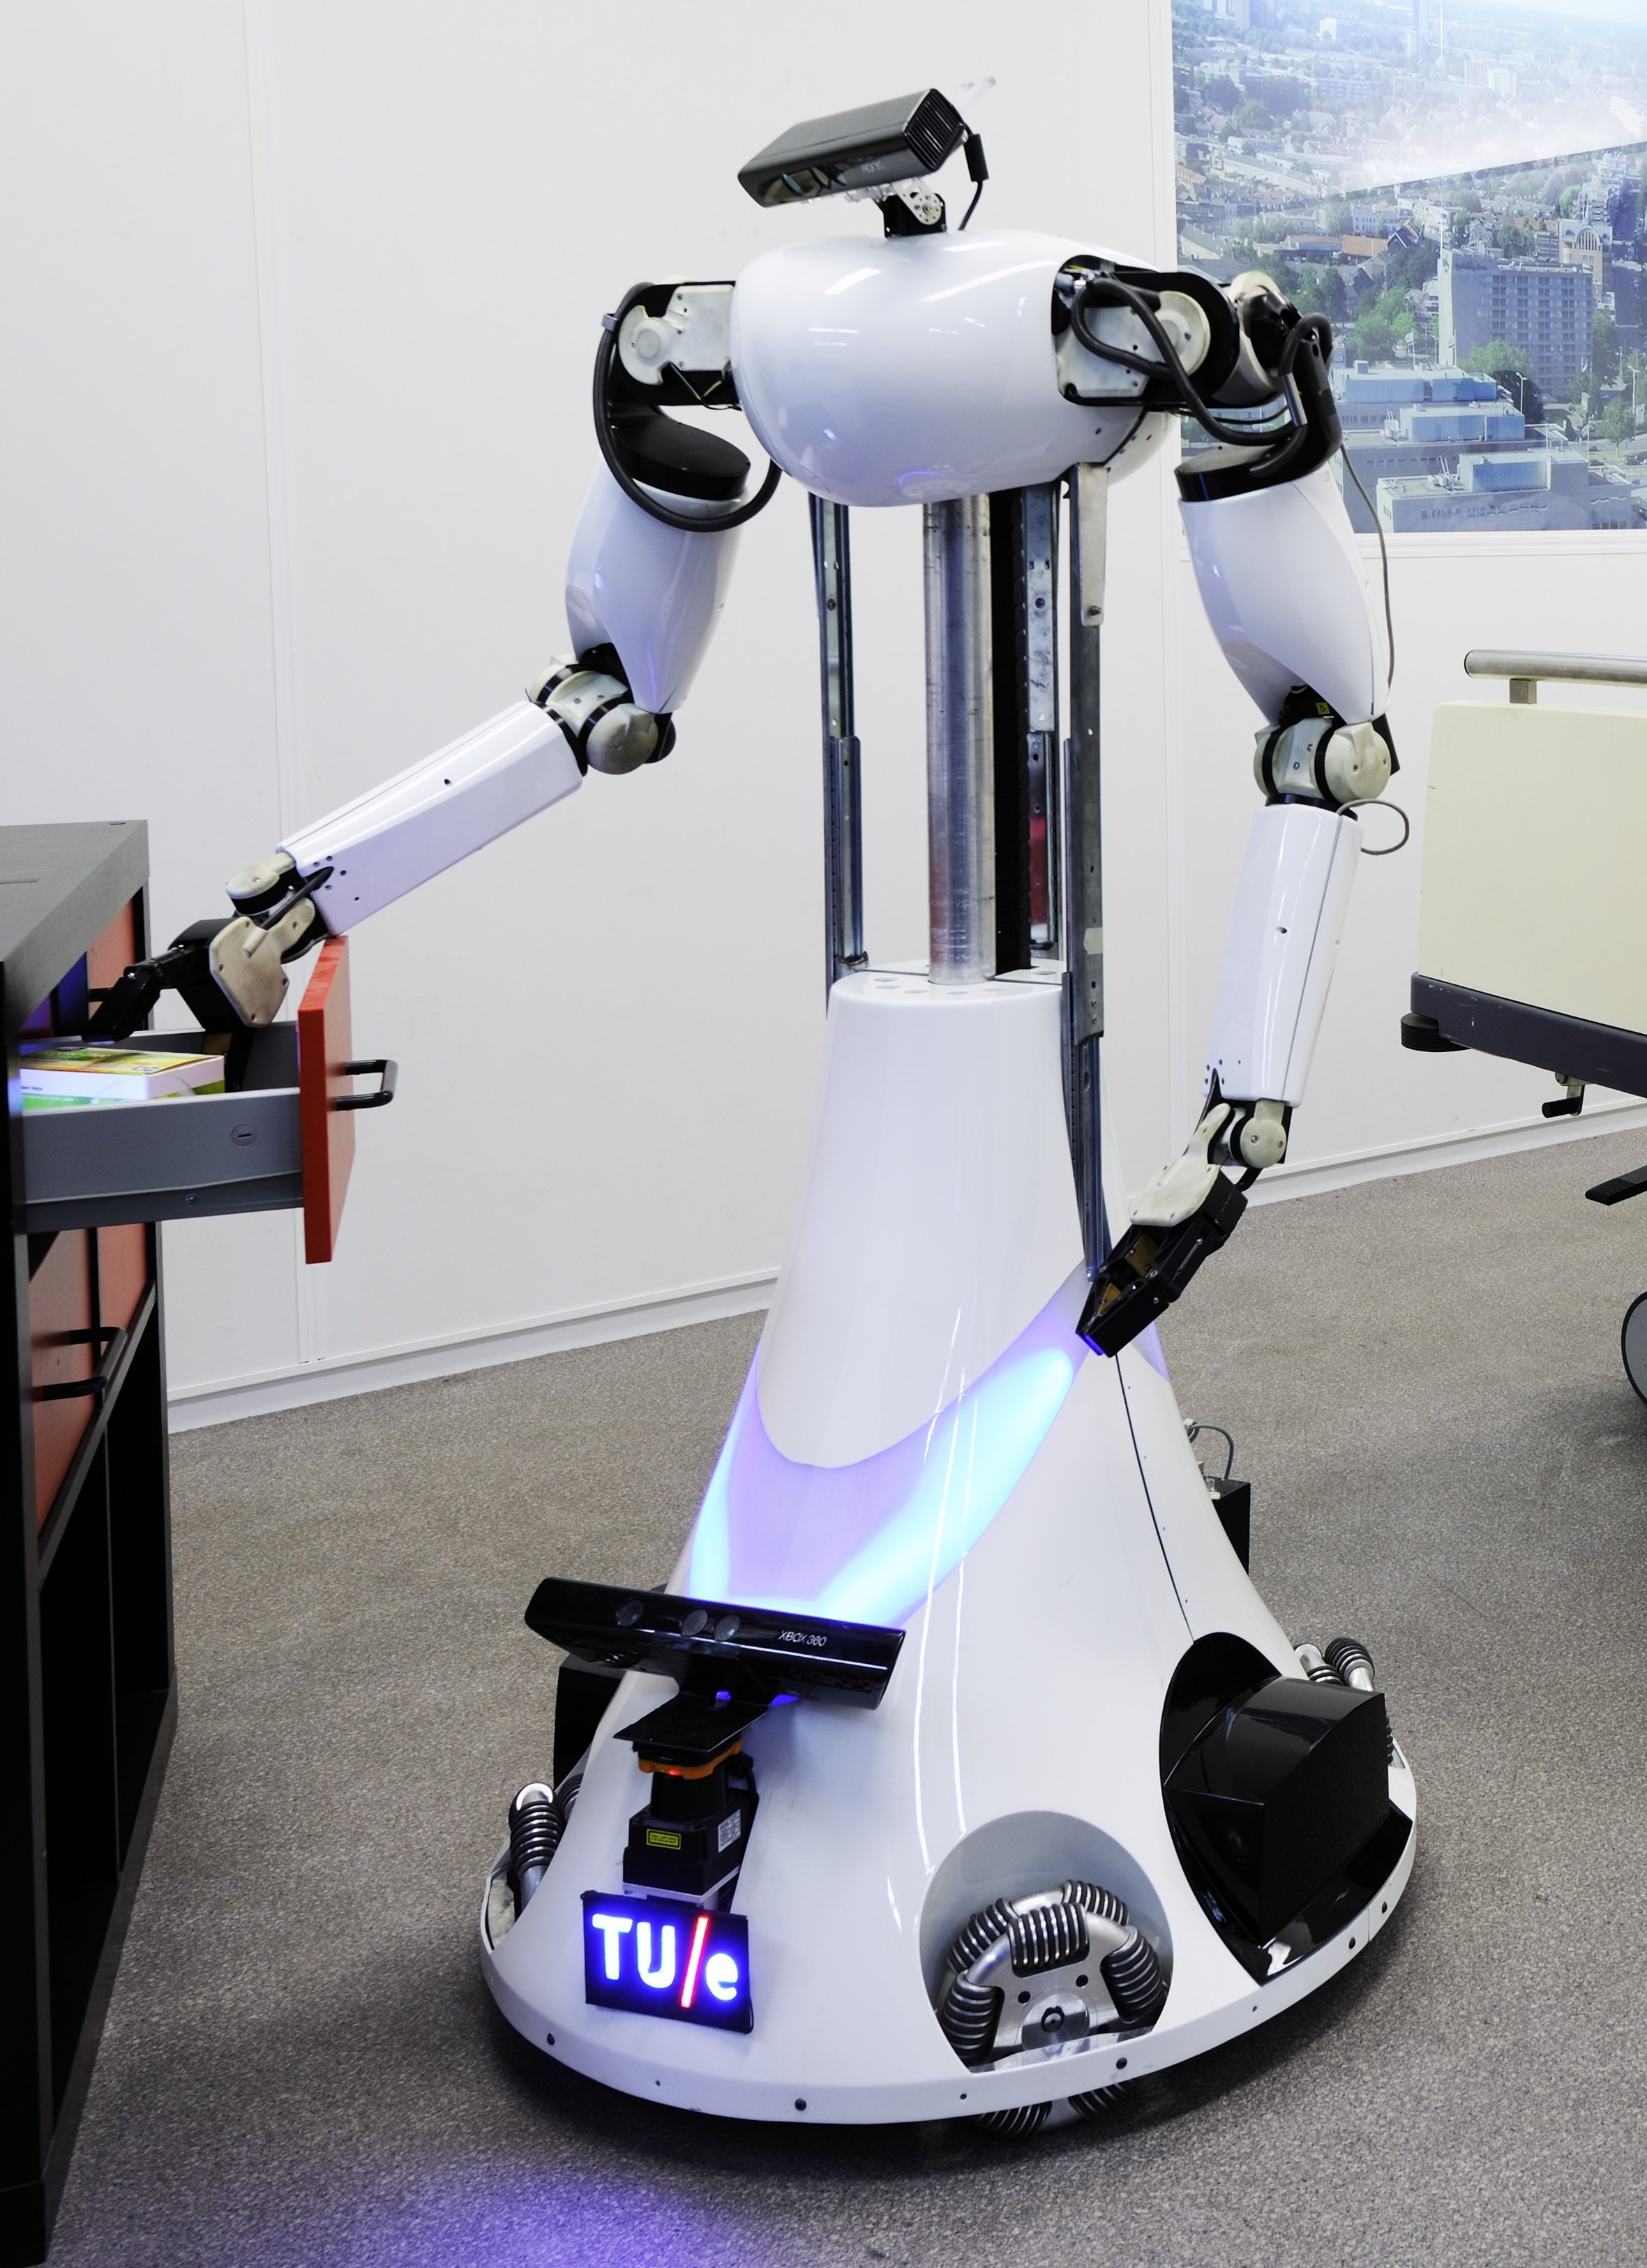
\includegraphics[width = 1\linewidth]{Figures/amigo_hospital72}\\
				AMIGO
            \end{center}
        \end{column}
        \hfill
        \begin{column}{0.4\textwidth}
            \begin{itemize}
                %\item Based on MSL TURTLE
                \item Holonomic base platforms
                %\begin{my_itemize}
                %    \item New wheels
                %\end{my_itemize}
                \item Moveable upper bodies
                \item 7-DoF manipulators
                %\item Two 7-DoF anthropomorphic arms
                %\begin{my_itemize}
                %    \item New electronics
                %\end{my_itemize}
                \item Designs on Robotic Open Platform
            \end{itemize}
            \begin{center}
                
\includegraphics[width = 0.75\linewidth]{Figures/LogoROP_v5}            
            \end{center}
        \end{column}
        \hfill
        \begin{column}{0.3\textwidth}
            \begin{center}
                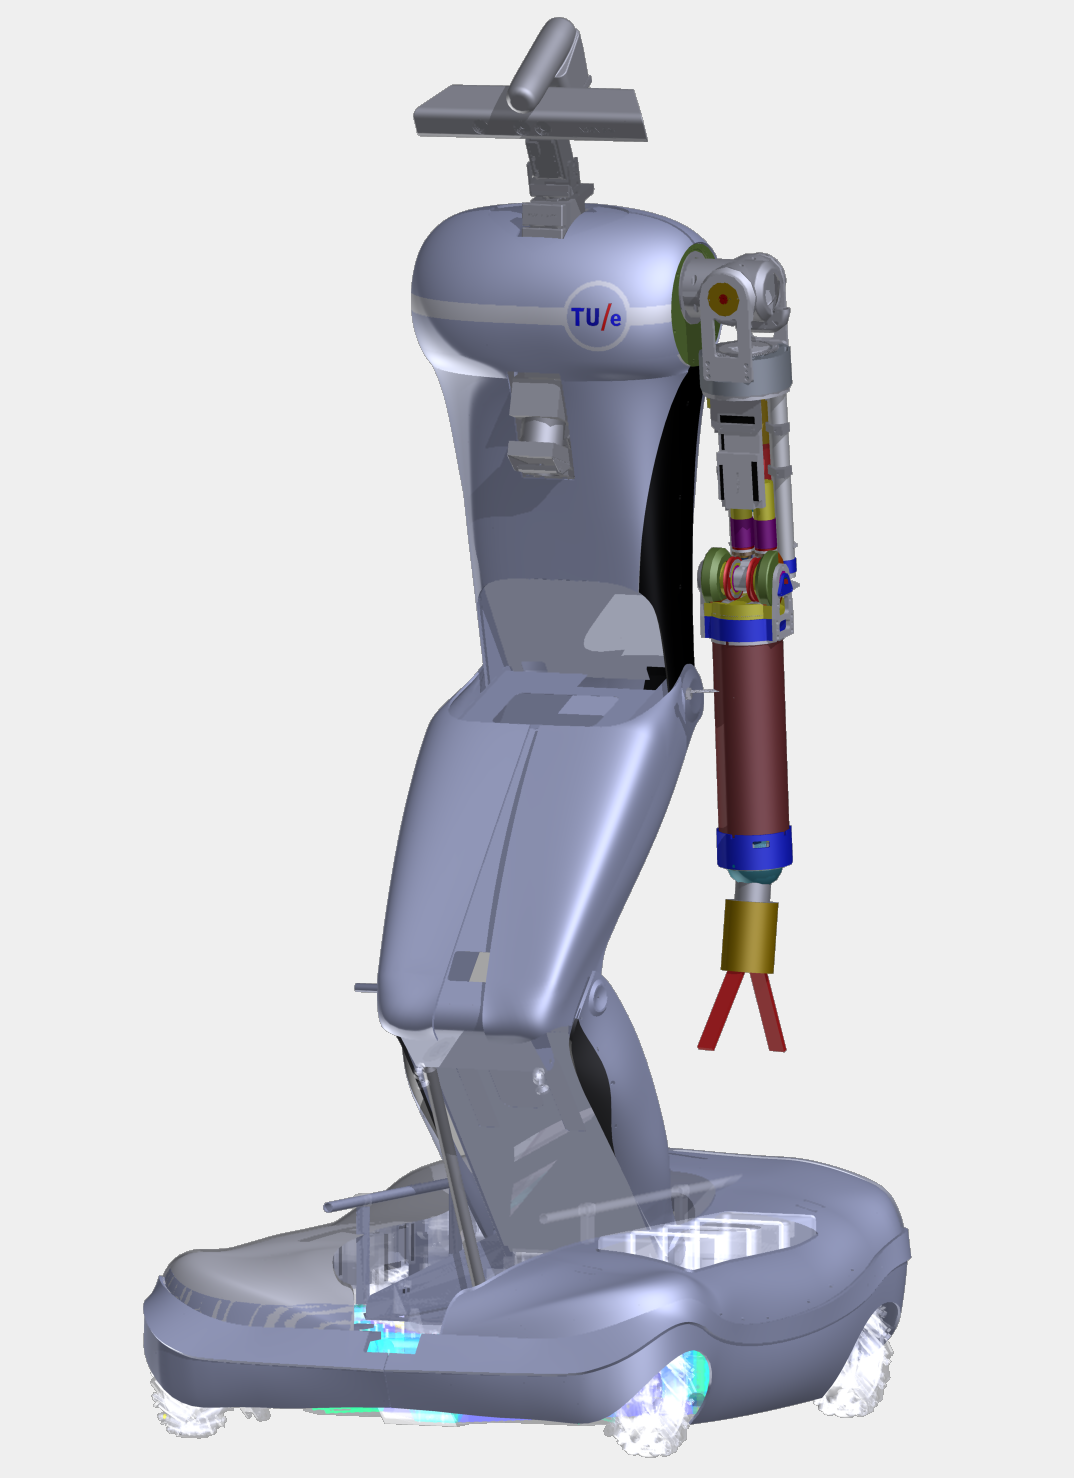
\includegraphics[width = 1\linewidth]{Figures/SERGIO}\\
                SERGIO
            \end{center}
        \end{column}
    \end{columns}
\end{frame}

\begin{frame}
	\frametitle{World modeling}
	\bigskip
	\begin{center}
		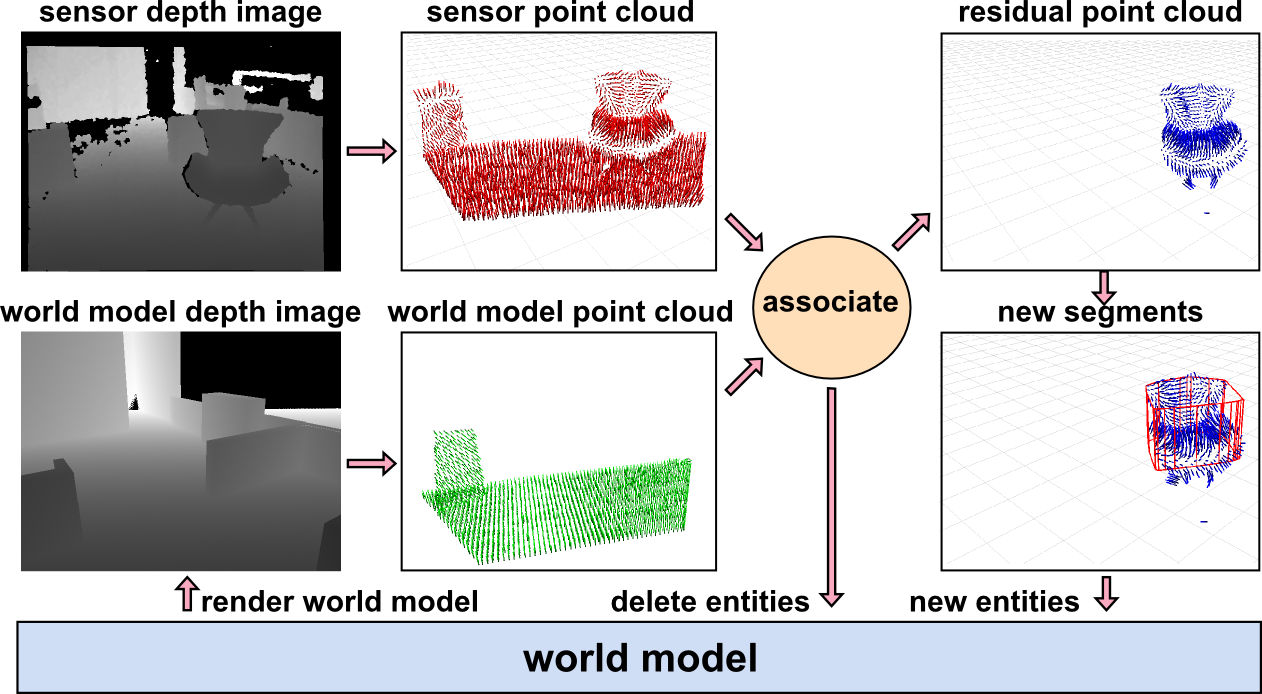
\includegraphics[width=0.8\linewidth]{Figures/ed_pipeline}
	\end{center}
\end{frame}

\begin{frame}
	\frametitle{Perception}
	\begin{columns}
		\begin{column}{0.33\textwidth}
			\begin{center}
				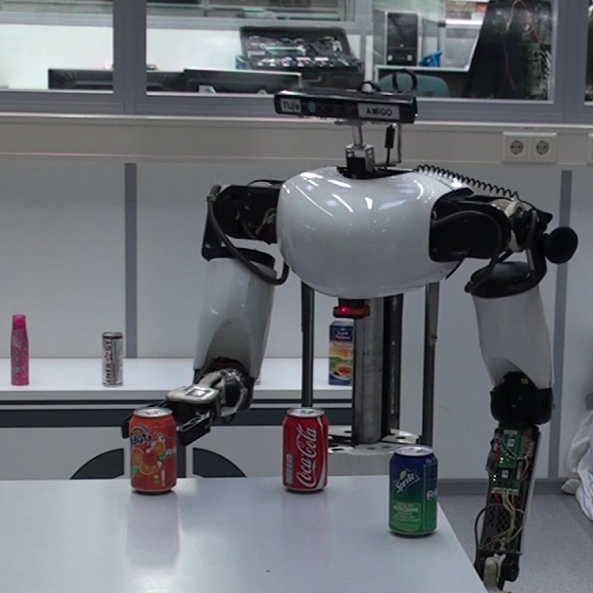
\includegraphics[width=1\linewidth]{Figures/pickup_object}\\
				Picking up an object
			\end{center}
		\end{column}
		\begin{column}{0.33\textwidth}
			\begin{center}
				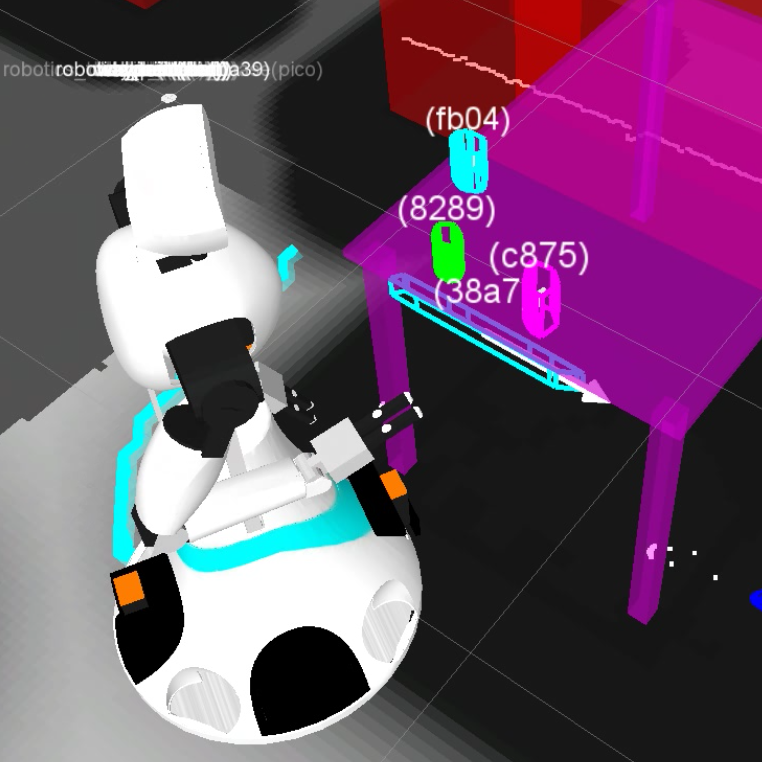
\includegraphics[width=1\linewidth]{Figures/pickup_object_world_model}\\
				World model view
			\end{center}		
		\end{column}
		\begin{column}{0.33\textwidth}
			\begin{center}
				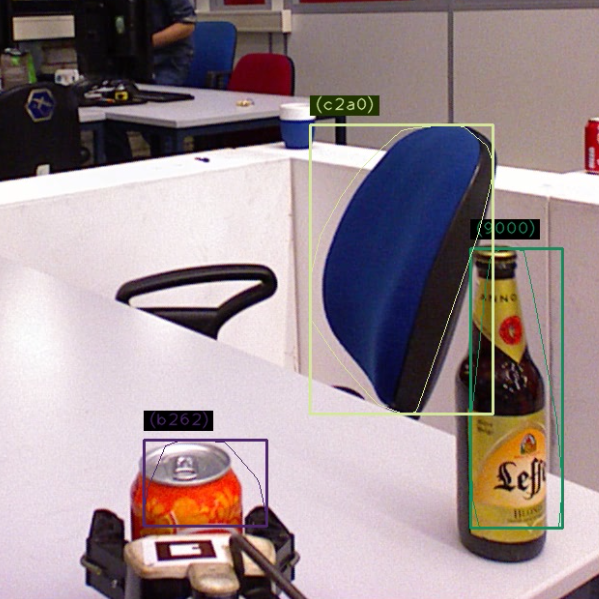
\includegraphics[width=1\linewidth]{Figures/pick_up_kinect_view}\\
				Sensor view
			\end{center}		
		\end{column}				
	\end{columns}
\end{frame}

\begin{frame}
	\frametitle{Navigation}
	\begin{columns}
		\begin{column}{0.5\textwidth}
			\begin{itemize}
				\item<1-> Navigation map: downprojection of world model entities
				\item<2-> Task dependent goal regions
				\item<3-> DWA planner with state behavior
			\end{itemize}
		\end{column}		
		\begin{column}{0.5\textwidth}
			\begin{center}
				\only<1> {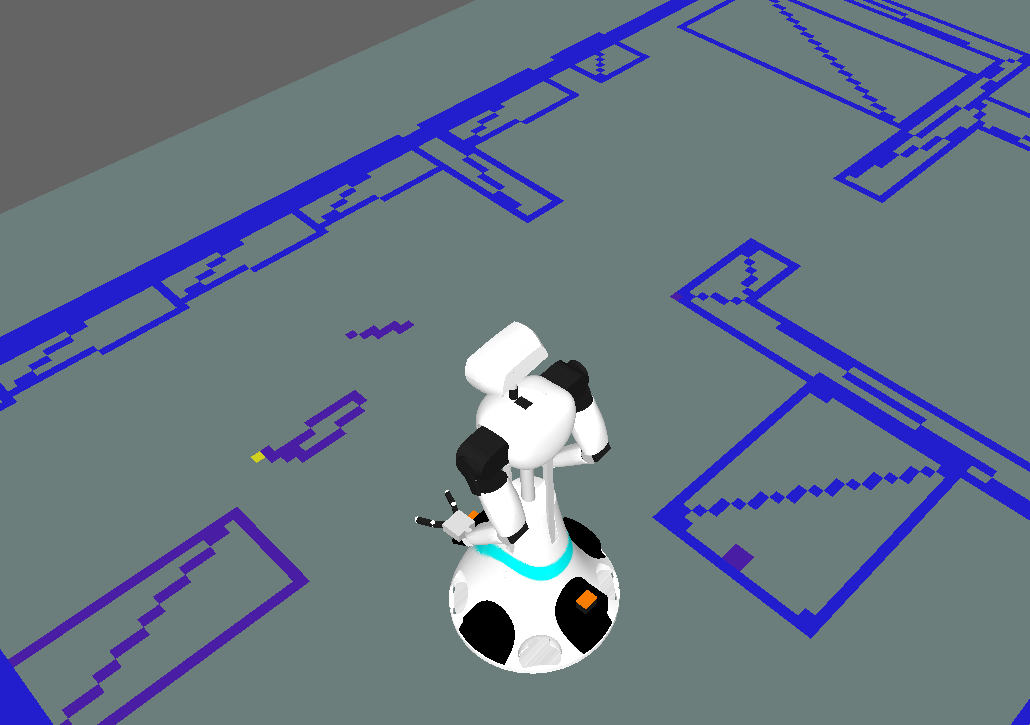
\includegraphics[width=1\linewidth]{Figures/lab_ed_map_crop}}
				\only<2-> {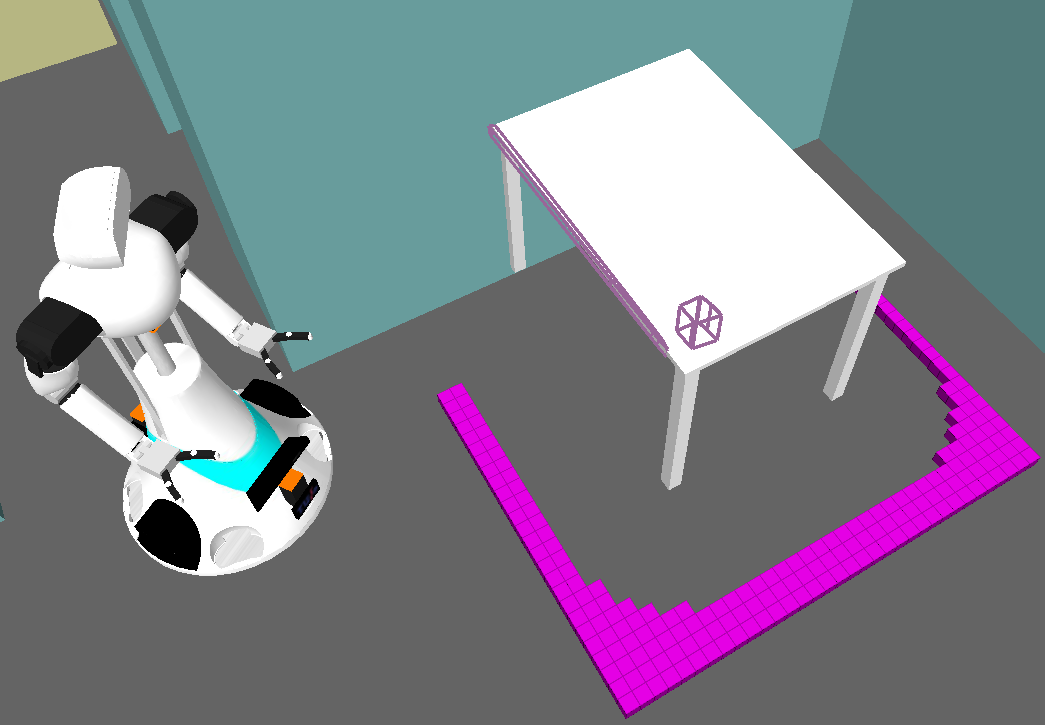
\includegraphics[width=0.75\linewidth]{Figures/constraint_table}
						  \\ \vspace{0.25cm}
						  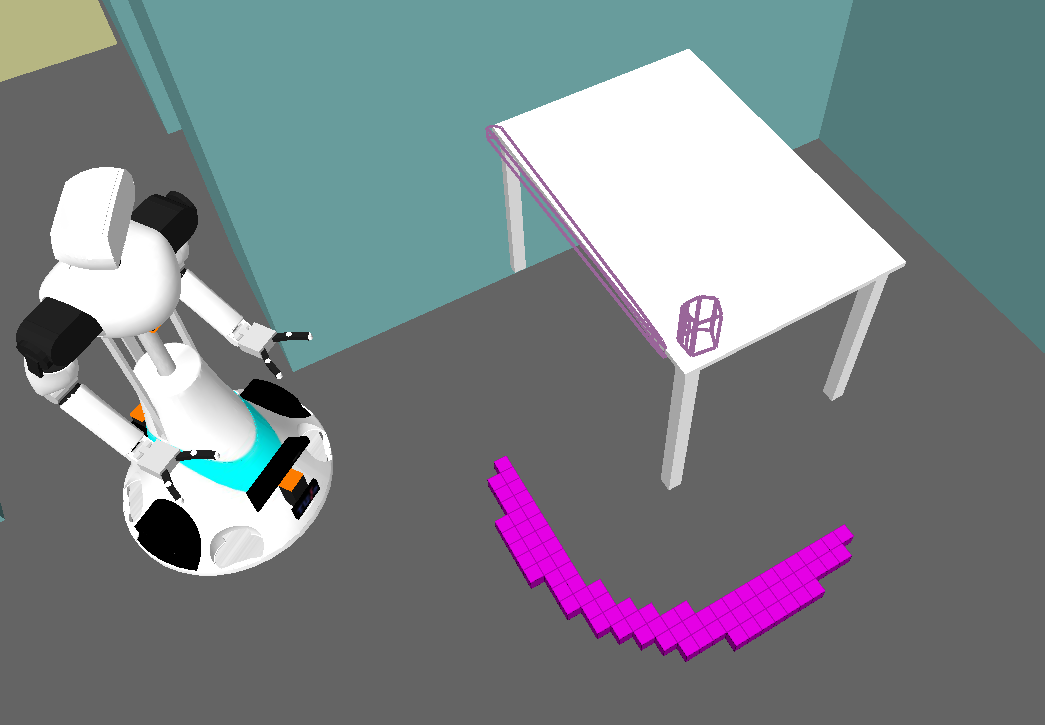
\includegraphics[width=0.75\linewidth]{Figures/constraint_grasp}}
			\end{center}
		\end{column}				
	\end{columns}
\end{frame}

%\begin{frame}
%    \frametitle{Motion Planning}
%    \begin{columns}
%        \begin{column}{0.5\textwidth}
%            \begin{itemize}
%            %    \item Determine the probability of a voxel being occupied by:
%            %    \begin{itemize}[itemsep = 0pt, parsep = 0pt, topsep = 0pt]
%            %        \item an object
%            %        \item the robot
%            %    \end{itemize}
%                \item Determine the probability of a voxel being occupied by either an object or the robot
%%                \begin{itemize}
%%                    \item probability of occupancy increases if no measurements are received to avoid over-confidence
%%                    \item unknown cells are inflated to account for occlusions
%%                \end{itemize}
%                \item Combine these probabilities% to compute the probability of collision
%                \item Determine a safe velocity limit% based on this probability
%                \item Current research: use semantic knowledge% to increase safety and socially desired behavior
%            \end{itemize}
%        \end{column}
%        \begin{column}{0.5\textwidth}
%        \vspace{-1cm}
%            \begin{center}
%                \begin{tikzpicture}
%        	      \tikzset{
%        		text label/.style={anchor=south east,font=\footnotesize, draw=none,fill=none,align=left,text=white, inner sep = 1pt, outer sep = 0pt},
%        		  small dot/.style={draw=white,thick,circle,scale=0.5},
%        		  every path/.style={draw=white,thick,line cap=round}
%        	      }
%        	      \node[anchor=south west,inner sep=0] at (0,0) {\includegraphics[trim = 0mm 45mm 0mm 0mm, clip, width=6cm]{Figures/rviz_screenshot_doorway.png}};
%        	      \node[text label](l3) at (6, 1.6) {\emph{p}$_\text{cell}=$ \emph{p}$_\text{max}$};
%        	      \node[small dot](l3_pin) at (1.88, 0.8){};
%        	      \path[draw] (l3.west) -- (l3_pin);
%        	      \node[text label](l2) at (6, 1.25) {\emph{p}$_\text{cell}=$ \emph{p}$_\text{min}$};
%        	      \node[small dot](l2_pin) at (2.55, 0.8){};
%        	      \path[draw] (l2.west) -- (l2_pin);
%        	      \node[text label](l1) at (6, 0.9) {\emph{p}$_\text{cell}=$ 0.5};
%        	      \node[small dot](l1_pin) at (3.35, 0.8){};
%        	      \path[draw] (l1.west) -- (l1_pin);
%        	   \end{tikzpicture}
%
%	           \def\svgwidth{6cm}
%	           \input{Figures/obst_infl.pdf_tex}
%            \end{center}
%        \end{column}
%    \end{columns}
%\end{frame}
%
%\begin{frame}
%    \frametitle{Reasoning and World Modeling}
%    %\bigskip
%    \begin{columns}
%        \begin{column}{0.5\textwidth}
%            \begin{itemize}
%                \item World model%: represents and maintains the properties of objects in the world
%                \item Reasoner%: contains knowledge to interpret properties and link them to predicates and facts
%                \item Executive%: queries the reasoner whenever information about the world is needed
%                \item Towards a volumetric world model:
%        %        \begin{itemize}
%        %            \item useful for motion planning
%        %            \item to prevent hardcoded waypoints and points of interest
%        %        \end{itemize}
%                \begin{itemize}
%                    %\item improve the estimated sensor pose
%                    %\item update the pose of possibly moving objects
%                    %\item remove unexplained objects from the world model
%                    %\item cluster unexplained sensor data and add it as an unknown object to the world model
%                    \item instead of hardcoded occupancy maps
%                    \item prevents hardcoded waypoints and points of interest
%                \end{itemize}
%            \end{itemize}
%        \end{column}
%        \begin{column}{0.5\textwidth}
%            \begin{center}
%                \includegraphics[width = 1\linewidth]{Figures/volumetric_world_model}
%            \end{center}
%        \end{column}
%    \end{columns}
%\end{frame}
%
%\begin{frame}
%    \frametitle{Perception}
%    \begin{columns}
%        \begin{column}{0.6\textwidth}
%            \begin{itemize}
%                \item Segment objects on top of a horizontal plane
%                \item Determine the size of these objects
%                \item Recognize textured objects using the objects of daily use finder perception system
%            \end{itemize}
%        \end{column}
%        \begin{column}{0.4\textwidth}
%            \begin{center}
%                \only<1>{\includegraphics[width = 1\linewidth]{Figures/tabletop}}
%                \only<2>{\includegraphics[width = 1\linewidth]{Figures/odufinder}}
%            \end{center}
%        \end{column}
%    \end{columns}
%\end{frame}

\end{document} 